
\documentclass[11pt]{article}
\usepackage[margin=0.5in]{geometry}
\usepackage[utf8]{inputenc}
\usepackage{setspace}
\setstretch{1}
\usepackage[english]{babel}
\usepackage[]{amssymb} 
%\usepackage[enable]{darkmode} 
\usepackage{amsmath, amsthm}
\usepackage{mdframed}
\usepackage{pgfplots}
\usepackage{booktabs}
\usepackage{enumitem}
\usepackage{hyperref}
\usetikzlibrary{pgfplots.fillbetween}  
\pgfplotsset{compat=1.17} 
\makeatletter
\newcommand{\tpmod}[1]{{\@displayfalse\pmod{#1}}}
\makeatother

\mdfdefinestyle{problemstyle}{
    innertopmargin=0pt,
    innerbottommargin=10pt,
    innerrightmargin=10pt,
    innerleftmargin=10pt,
    outerlinewidth=1pt,
    topline=true,
    bottomline=true,
    leftline=true,
    rightline=true
}

%custom enviroment for exercises
\newenvironment{exercise}{
    \begin{mdframed}[style=problemstyle]\textcolor{black}{}
}{
    \end{mdframed}
}


\title{TMATH 126 Midterm Review Workshop}
\author{}
\date{\vspace{-5ex}}

\begin{document}
\maketitle
\vspace{-5ex}%not a fan of this, but good fix for now

Unless otherwise stated let $\vec{u} = \langle 2,-3,5 \rangle$ and 
$\vec{v} = \langle 4, -1, 2 \rangle $ 
\subsection*{1a: Coordinates and Vectors in 2D and 3D}
\begin{exercise}
    \begin{enumerate}[label={\alph*}]
        \item Draw vectors $\vec{u}$ and $\vec{v}$ in 2D and 3D. 
            Then draw $\vec{u} + \vec{v}$ using the tip-to-tail method.
        \item Draw and label $\vec{u} - \vec{v}$ on the same coordinate 
            system.
    \end{enumerate}
\end{exercise}

\subsection*{1b: Dot Product, Cross Product}
\begin{exercise}
    \begin{enumerate}[label={\alph*}]
        \item Explain the applications of the dot and cross product.
            (ie what do they tell/give us)
        \item Find the scalar projection of $\vec{u}$ onto $\vec{v}$.
        \item Find the vector projection of $\vec{v}$ onto $\vec{u}$.
        \item Find the angle between $\vec{u}$ $\vec{v}$.
        \item Find the area of a parallelogram with the points $A(0,1,3)$, 
            $B(1,3,5)$, $C(5,7,5)$, $D(4,5,3)$.
    \end{enumerate}
\end{exercise}

\subsection*{1c: Equations of Lines and Planes}
\begin{exercise}
    \begin{enumerate}[label={\alph*}]
        \item Given point $A(1,1,1)$ and $\vec{d} = \langle 10, -10, 50 \rangle$
            Write the vector equation of a line in 2D and 3D that contains point $A$ 
            moves is parallel to $\vec{d}$.
        \item Find the equation of a plane with points $(4, -3, 1)$, $(-3,-1, 1)$,
            and $4,-2, 8$.
        \item Determine if the planes given by $4x - 9y - z = 2$ and 
            $x + 2y -14z = -6$ are parallel, orthogonal, or neither.
        \item Determine where the line $\vec{r}(t) = \langle -2t, 2+7t, -1-4t \rangle$
            and the plane given by $\langle 4x + 9y - 2z = -8$ 
        \item Find the line of intersection of the planes given by 
            $3x + 6y - 5z = -3$ and $-2x + 7y - z = 24$.
        \item Find the point on the plane $3x + 4y + z = 1$ that is closest to the 
            point $(1, 0, 1)$.
    \end{enumerate}
\end{exercise}

\newpage
\subsection*{1d: Equations of Cylinders and Other Simple Surfaces}
\begin{figure}[!ht]
    \centering
    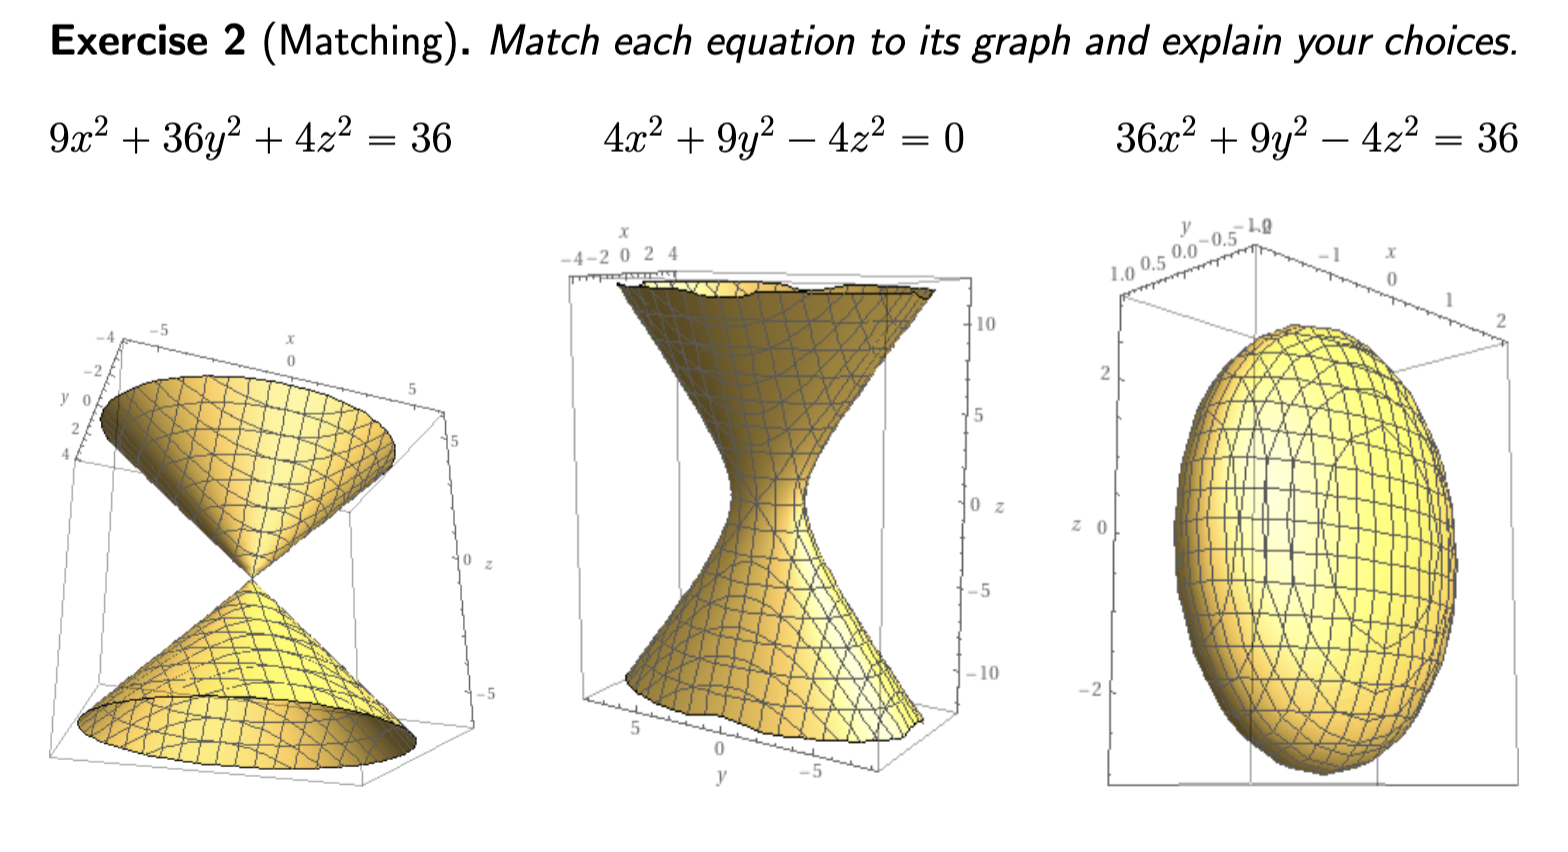
\includegraphics[width=0.5\textwidth]{images/match-practice.png}
\end{figure}
\begin{exercise}
    Identify and sketch the following 3D surfaces.
    \begin{enumerate}[label={\alph*}]
        \item $x^2 + y^2 + z^2 = 1$
        \item $x=cost$ and $y=sint$
        \item $x^2 +\frac{y^2}{9} + \frac{z^2}{4}$
        \item $z=4z^2+y^2$
    \end{enumerate}
\end{exercise}


\end{document}

